\documentclass[usenatbib]{mnras}

\usepackage{silence} % silence error warinings
\WarningFilter{caption}{Unsupported document class} % caption doesn't know mnras..
\hbadness = 5000
\vbadness = 10000

% Don't change these lines unless you know what you are doing
\usepackage[T1]{fontenc} % make sure font is supported
% \usepackage{ae,aecompl} %obsolete when using modern fonts
\usepackage[final]{microtype} % make sure font is supported
% and a suitable font
\usepackage{lmodern} % use a modern font with T1 support
%\usepackage{cm-super} % use a modern font with T1 support

\usepackage{graphicx} % Including figure files
\usepackage{amsmath}	% Advanced maths commands
\usepackage{amssymb}	% Extra maths symbols
\usepackage{pifont}	% Extra maths symbols
\usepackage{hyperref}   % Hyperlinks
\hypersetup{colorlinks=true,linkcolor=blue,citecolor=blue,filecolor=blue,urlcolor=blue}

\title[Short title]{Long title}

\author[Oswald et al]{Lucy Oswald,$^1$
Andreas Sch\"arer$^2$ and Prasenjit Saha$^2$\\
%
$^1$Murray Edwards College, University of Cambridge, Cambridge CB3 0DF, UK\\
$^2$Physik-Institut, University of Zurich, Winterthurerstrasse 190, 8057 Zurich, Switzerland\\
}

% These dates will be filled out by the publisher
% \date{Accepted XXX. Received YYY; in original form ZZZ}

\pubyear{2016}

% Don't change these lines
\begin{document}
\label{firstpage}
\pagerange{\pageref{firstpage}--\pageref{lastpage}}
\maketitle

\begin{abstract}
\end{abstract}

\begin{keywords}
\end{keywords}

\section{Introduction}

Recent years have seen exciting examples of relativistic
orbits \citep{2006Sci...314...97K,2006NewA...11..527C,2011PhRvL.106v1101E}.

Galactic-centre black hole also attracted attention
\citep{2008ApJ...674L..25W,2010ApJ...711..157A,2010ApJ...720.1303A,2015ApJ...809..127Z}.
Unfortunately, not a clean system \citep[cf.][]{1947RvMP...19..361C}.
Wavelet filtering one idea \citep{2014MNRAS.444.3780A}.  Here we
propose another.

Filter functions $\phi_k(t)$ which we apply to noisy signal $z(t)$ to
get filtered signal $\bar z(t)$.
\begin{equation}
\begin{aligned}
        a_k &= \int\! z(t)\,\phi_k^*(t)\,dt \\
  \bar z(t) &= \sum_k a_k \, \phi_k(t) .
\end{aligned}
\end{equation}
Formulated as complex because convenient for our toy model later.

\section{Method}

\citep{chatterjee2000introduction}

\begin{equation}
C_{mn} = \int\! z_m(t)\,z_n^*(t)\,dt
\end{equation}

\begin{equation}
C_{mn} = \sum_p E_{mk} \, \lambda_k^2 \, E_{kn}^*
\end{equation}

\begin{equation}
S_k(t) = \frac{\sum_n E_{kn}^*\,z_n(t)}{\lambda_k}
\end{equation}

\begin{equation}
w_k(t) = S_k(t) - \sum_l \int\! S_k(t)\,B_l^*(t)\,dt
\end{equation}

\section{A toy model}

\def\half{\mbox{$\frac12$}}
\begin{equation}
\begin{aligned}
H(x, y, p_x, p_y) =\,& \half \left( p_x^2 + p_y^2 \right)
                   - \half (1-2M/r)^{-1}                   \\
                  &- M (xp_x+yp_y)^2 / r^3\,,
\end{aligned}
\end{equation}
where $r=\sqrt{x^2+y^2}$.
\begin{equation} \label{dot-t}
     \dot t = (1 - 2M/r)^{-1} \,.
\end{equation}

\begin{equation}
H_1 = m_1
  \left( \frac{{\bf r\cdot r}_1}{|{\bf r}_1|^3}
         - \frac1{|{\bf r} - {\bf r}_1|} \right)  \,.
\end{equation}

\begin{figure*}
\centering
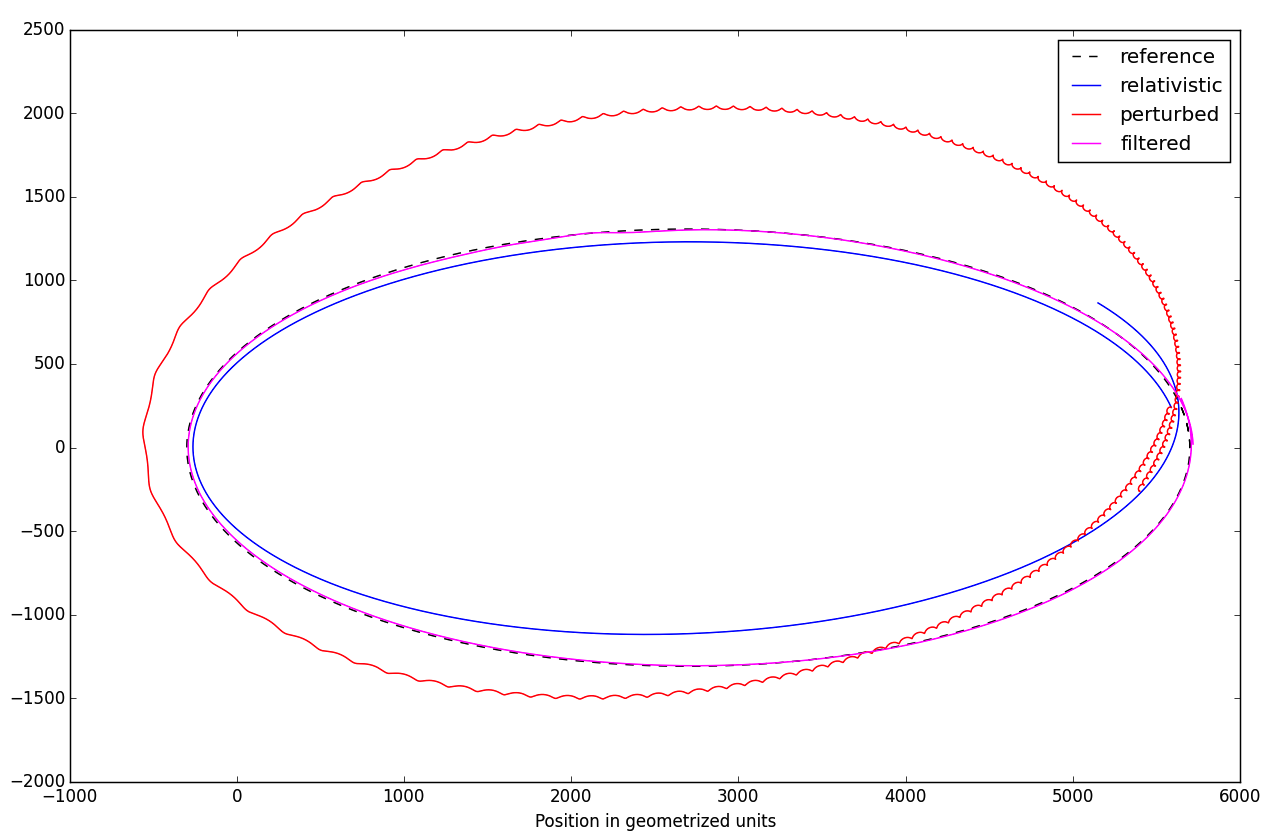
\includegraphics[height=.5\hsize]{orbits.png}
\caption{\label{fig:orbits} Filtering an orbit.}
\end{figure*}

\begin{figure*}
\centering
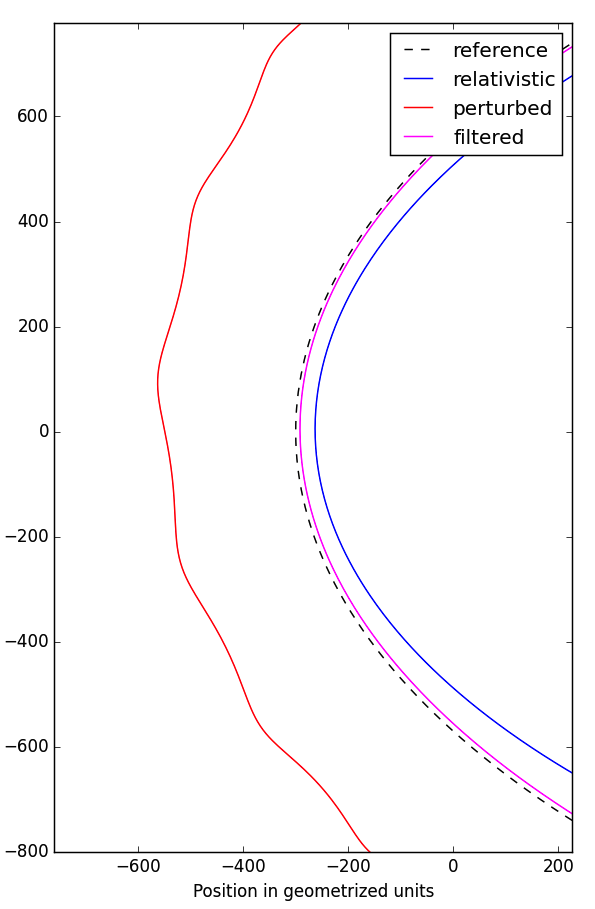
\includegraphics[height=.5\hsize]{zoom-peri.png}\quad
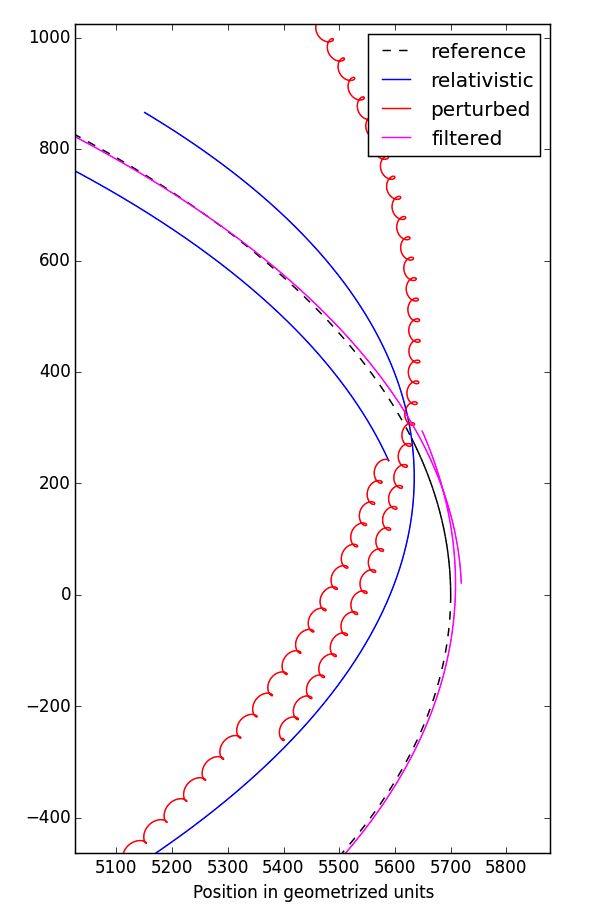
\includegraphics[height=.5\hsize]{zoom-apo.png}
\caption{\label{fig:zoom} Zoom of Figure~\ref{fig:orbits}.}
\end{figure*}

\bibliographystyle{mnras}
\bibliography{many}

% Don't change these lines
\bsp    % typesetting comment
\label{lastpage}
\end{document}

